%%%%%%%%%%%%%%%%%%%%%%%%%%%%%%%%%%%%%%
% Contribution to IKP annual report 2021
%%%%%%%%%%%%%%%%%%%%%%%%%%%%%%%%%%%%%%
\documentclass[fleqn,twocolumn,a4paper]{ikpar}
\usepackage{hyperref}
\usepackage{paralist}
\usepackage{times,mathptm}
\usepackage{graphicx}
\usepackage{float}
\usepackage{caption}
\usepackage{subfig}
\usepackage{gensymb}
\pagestyle{empty}

% standadized SI units
\usepackage[per-mode=symbol, range-units=single, binary-units=true]{siunitx}
\DeclareSIUnit\clight{\text{\ensuremath{c}}} % redefine light speed symbol
\DeclareSIUnit\momentum{\GeV\per\clight} % momentum in GeV/c
\DeclareSIUnit\tmom{(\momentum)^2} % 4-momentum squared
\DeclareSIUnit\atom{\text{atoms}} 
\DeclareSIUnit\event{\text{events}} 

% \addtolength{\topmargin}{-0.2cm}
% \addtolength{\textheight}{0.2cm}
\begin{document}
\parindent=0pt
\frenchspacing

\title{{\bf
    Determination of the cluster target density profile in KOALA
}}
\author{Yong Zhou
}

\maketitle

%%%% Background, problem description, topic and results of this report
KOALA aims to measure the differential cross section of (anti)proton-proton elastic
scattering over a wide $|t|$ range from \SIrange{0.0008}{0.1}{\tmom}.
In the initial setup, in which only the recoil detector is commissioned, the high yield of low-energy
background detererioates the elastic peak identification at small recoil angles and limits the lower measurement range of KOALA.
The forward detector, which is made from fast scintillators, has been built and
commissioned in 2019 to help supressing the low energy background based on TOF-E
relation of the recoil protons.
The design of the forward detector has been veried in the following test runs and energy spectrums from pure elastic scattering events can now be obtained after the TOF-E selection.
Due to the lower limit of the acceptance of the forward detector, the spectrums
of strips at very small recoil angles start to lose some events from the
target body beyond a threshold angle.
However, it is found that this phenomenon appears at a larger recoil angle than the design goal.
This is caused by the unexpected large thickness of the cluster target along the beam axis.
Thus, it's important to get more accurate information about the target profile.
In this report, a new method of determining the density profile of the cluster
target in KOALA is described, and the result from the 2019 beam test is presented.
The implication of measured target profile on the lower limit of KOALA measurement range is also discussed.

\par
\medskip

%%%%% Description of the method
The target thickness can be ignored at large recoil angles, since the strips are
far away from the interaction point.
This assumption does not hold for strips located close to the interaction point.
Three scenerios are depicted in Fig. \ref{fig:target_density_determination} to
show the variation of the measured energy spectrums with respect to smaller
recoil angles.
The acceptance of the forward detector covers the fully target body in the
beginning (Fig. \ref{fig:target_density_determination} (1)), it gradually losts part of the target body
(Fig. \ref{fig:target_density_determination} (2)), then the peak, and finally only covers
the tail of the target body (Fig. \ref{fig:target_density_determination} (3)).
In the end, it losts the target body completely and only measures the residual
gas contribution.
\begin{figure*}[h!]
  \centering
	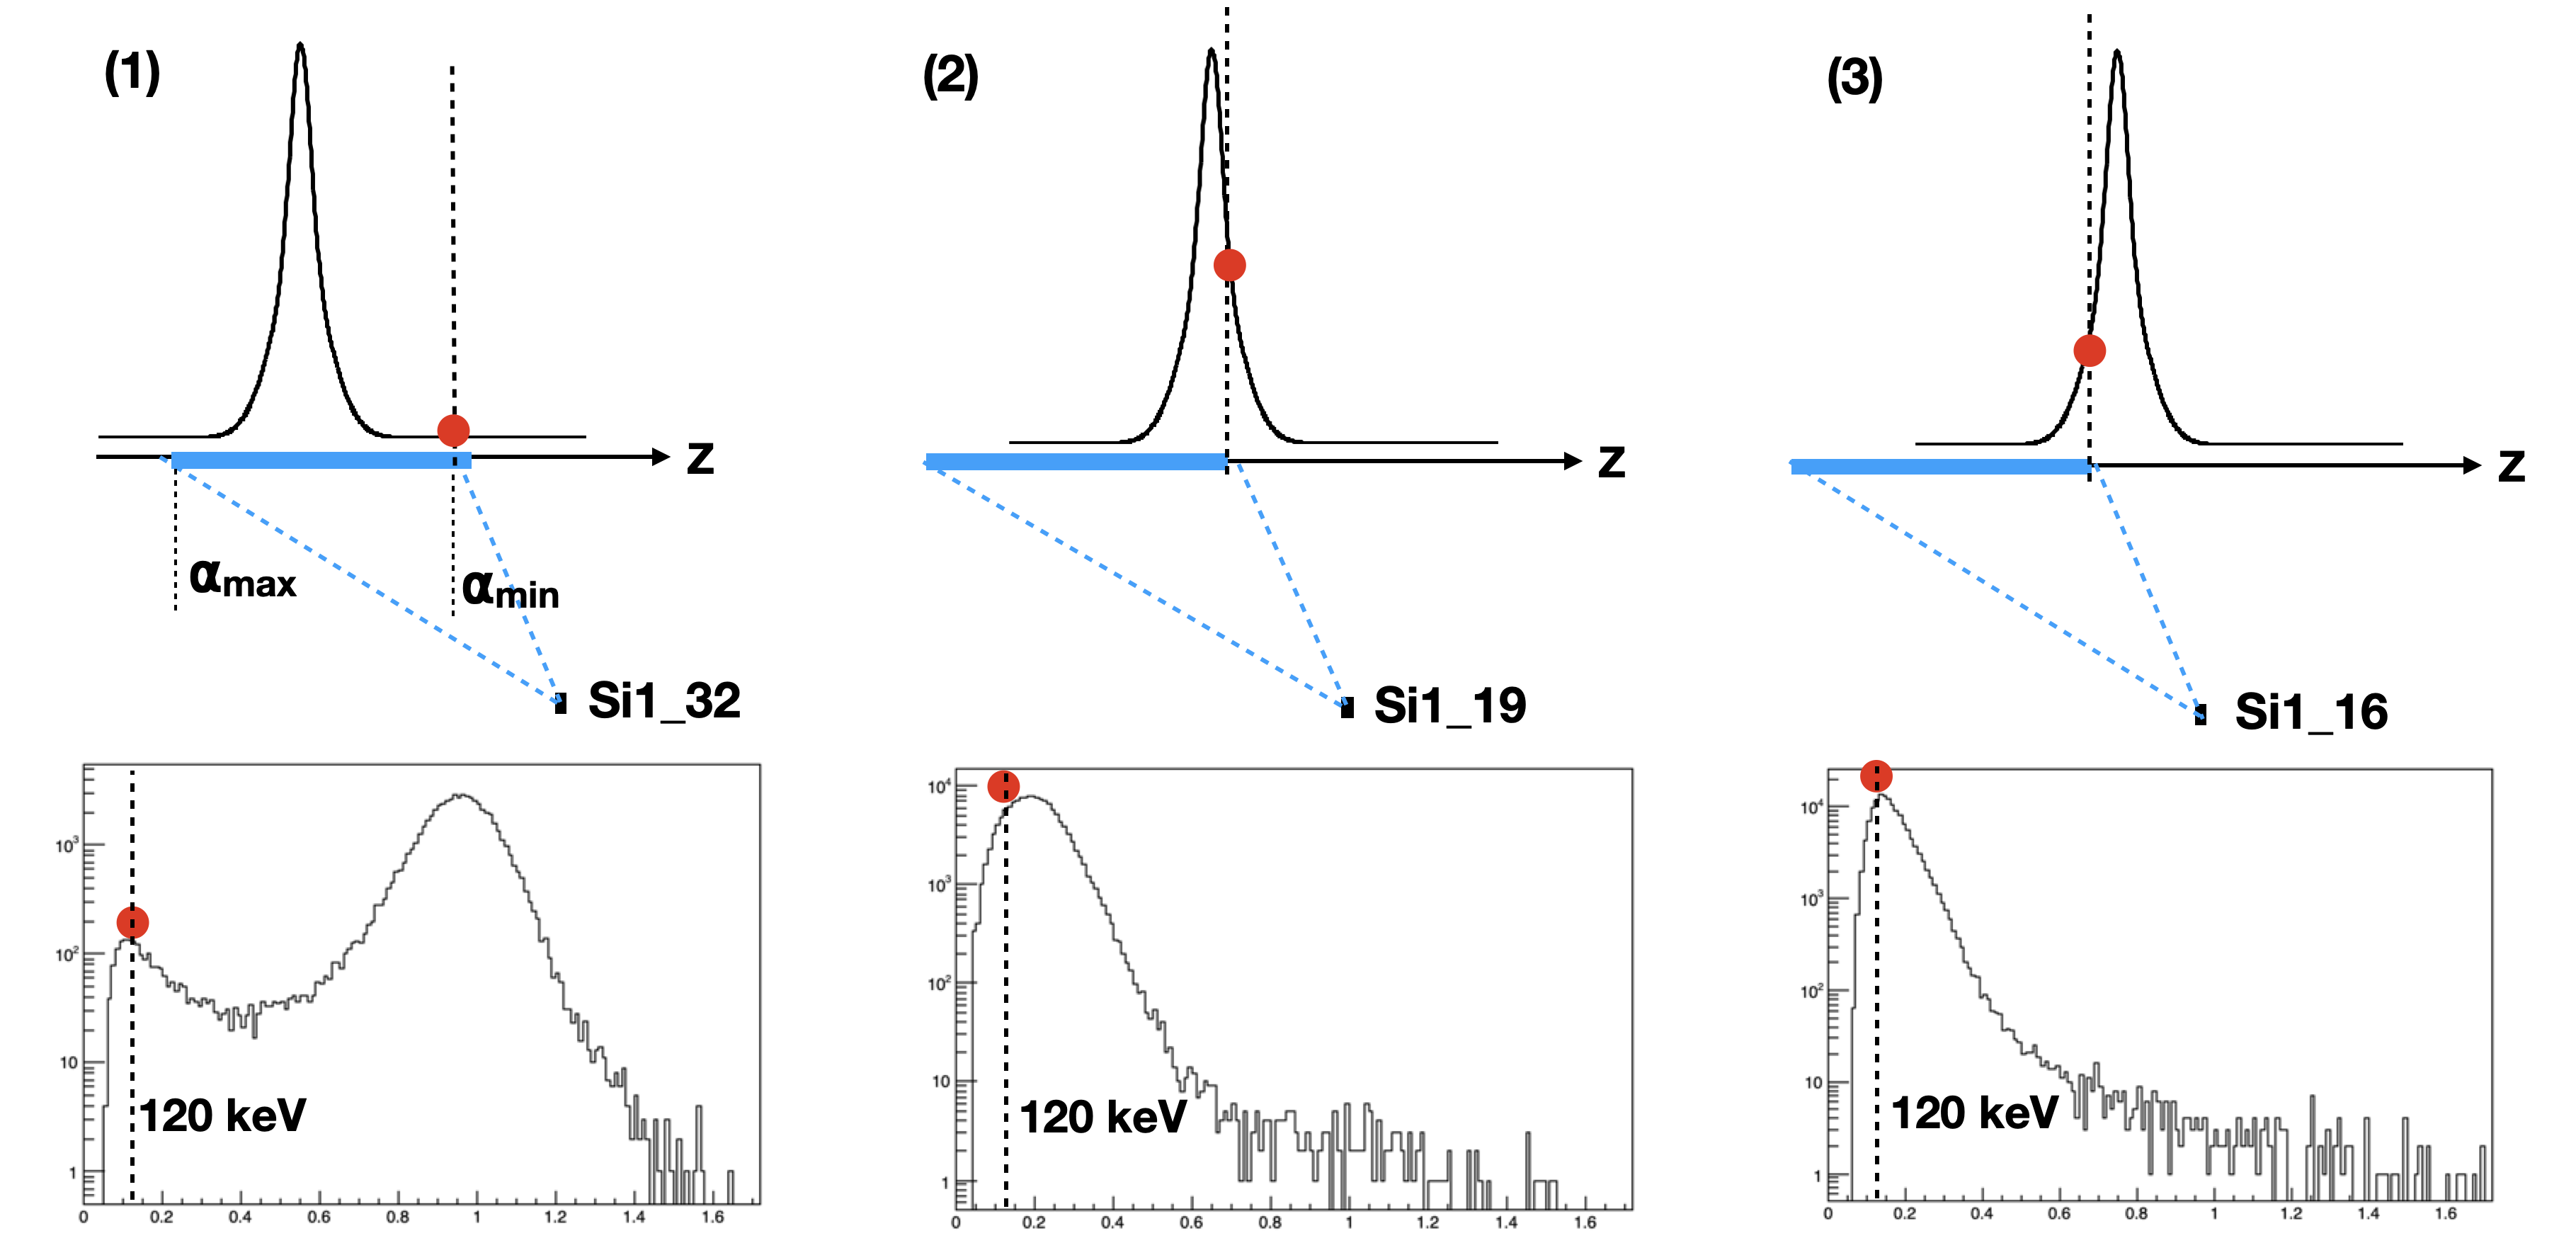
\includegraphics[width=0.8\textwidth]{./target_density_determination.png}
  \caption{Three scenerios showing the variation of recorded elastic energy
    spectrums measured by three strips at different recoil angles: (1) the full
    target body is within the acceptance of the
    forward detector; (2) part of the target body is not within the
    acceptance, but target center is still covered; (3) the target center is out of the
    acceptance, only the tail of the target profile is recorded. The first row
    shows the target profile shape and the second row is the measured energy
    spectrum at each recoil angle. The blue bar indicates the region covered by
    the forward detector and the red dot indicates the reference energy bin and
    its corresponding position in the target profile.}
  \label{fig:target_density_determination}
\end{figure*}

The number of TOF-E selected elastic scattering events $N_{elastic}$ recorded on a single recoil strip has the
following relation with other experiment parameters,
\begin{equation}
  N_{elastic} = \epsilon_{DAQ}\cdot l_{beam}\cdot\rho_{target}\cdot\sigma_{elastic}\cdot\epsilon_{acceptance}
\end{equation}
where $\epsilon_{DAQ}$ is the DAQ efficiency, $l_{beam}$ is the beam intensity, $\rho_{target}$ is the target density,
$\sigma_{elastic}$ is the cross section of elastic scattering and
$\epsilon_{acceptance}$ is the acceptance of the forward detector.
$l_{beam}$ and $\epsilon_{DAQ}$ are constant in the same run.
To determine $\rho_{target}$, the last two items $\sigma_{elastic}$ and
$\epsilon_{acceptance}$ need to be fixed.
$\sigma_{elasitc}$ is determined by the energy of the recoil proton, thus can be
fixed by choosing the same energy value as reference.
$\epsilon_{acceptance}$ varies with the recoil angle as well as the beam size.
Simulation shows that strips at the lower range of the forward coverage are
guaranteed to be fully covered as long as the width of the beam profile is
smaller than \SI{10}{mm}, see Fig. \ref{fig:fwd_acceptance}.
Since the strip corresponds to a specific recoil angle which in turn
can be converted to an energy value, this indicates that the elastic events with recoil energy close to the lower
limit of the forward detector's acceptance range are guaranteed to be fully covered and has $\epsilon_{acceptance} = 1$.
Thus, the event number in the energy bins close to the edge of the energy
spectrum changes only with $\rho_{target}$ and can be used directly as the relative measurement of the target density.
For \SI{2.2}{\momentum} run data, the observed lower limit of the forward
acceptance is about \SI{100}{\keV}.
The value is consistent with the calculated range of the forward detector's
acceptance with ideal beam condition, which is from \SIrange{0.096}{1.56}{\MeV}.
Thus, \SI{120}{keV} with bin width of \SI{10}{\keV} is selected at the
measurement reference.
\begin{figure}[htb!]
  \centering
	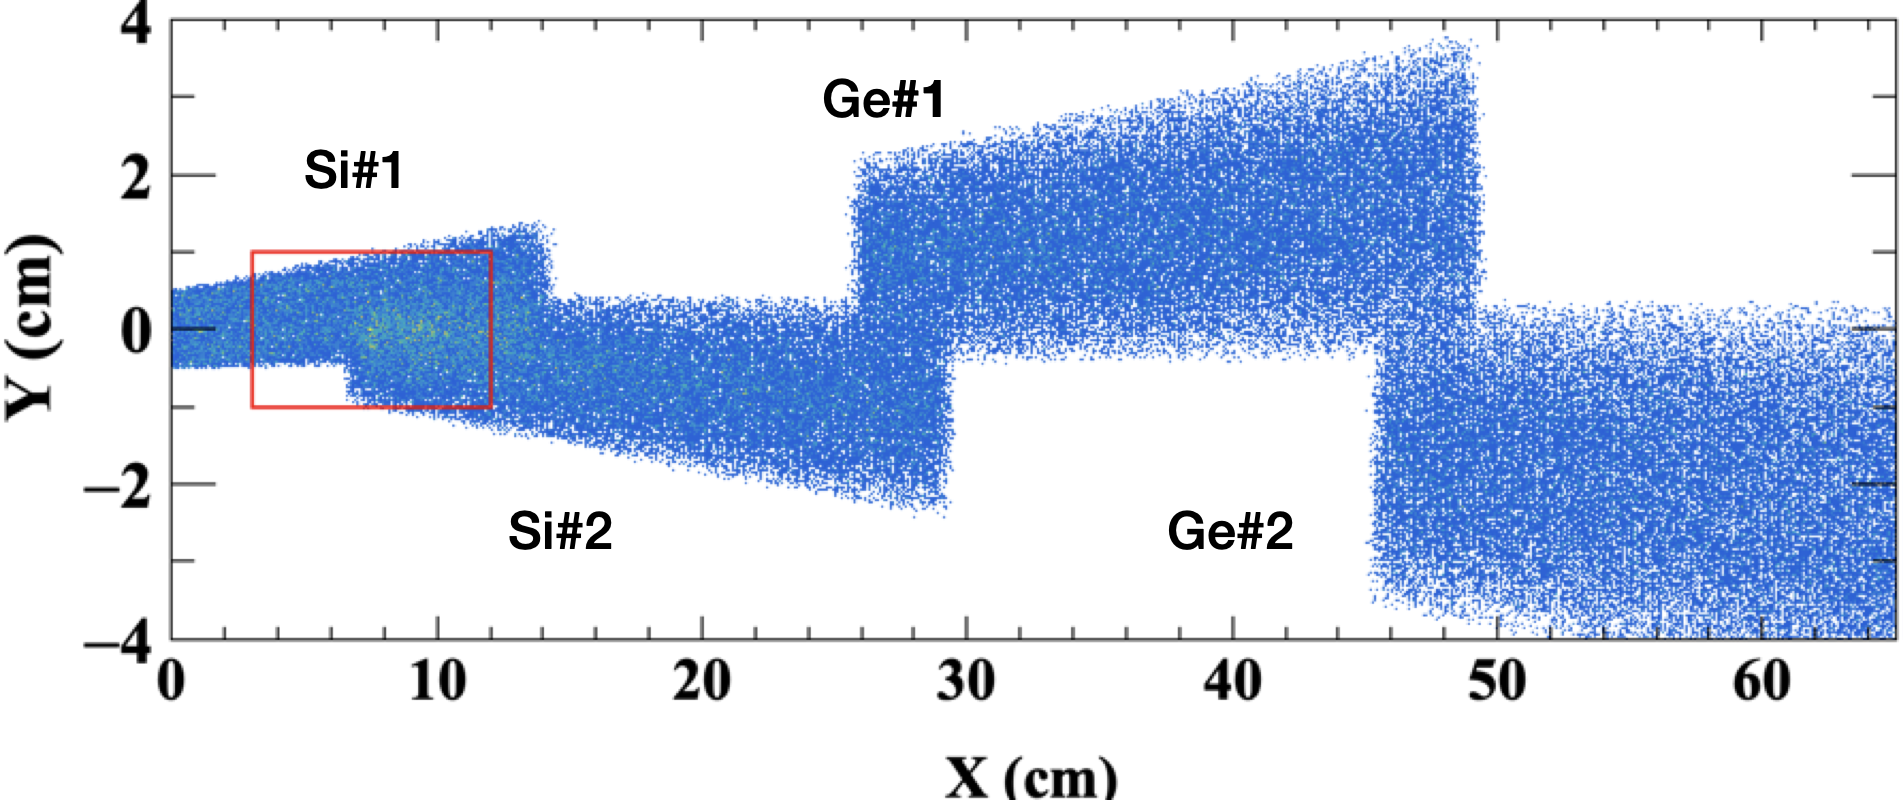
\includegraphics[width=0.5\textwidth]{./fwd_acceptance.png}
  \caption{Acceptance of the forward detector from the simulation using a square
    beam with \SI{10}{\mm} width. The blue blocks are the hit map on the forward
    detector plane for events hitting the recoil sensors. The red square indicates
    the size of the forward scintillators.}
  \label{fig:fwd_acceptance}
\end{figure}

\par
\medskip

The target density profile along the beam axis is measured by recording the event counts of the same energy bin in all strips.
The reference energy is converted back to a position before the strip center
(at \SI{2.2}{\momentum} beam momentum,\SI{120}{\keV} corresponds to \SI{10}{\mm}).
This process is also shown in Fig.\ref{fig:target_density_determination}.
Two independent methods are used to deduce the position distribution of the density profile.
The first method is based on the strip position in the ideal geometry model.
This method gives density distribution in the laboratory reference frame.
The second method is based on the energy difference of the reference energy and
the peak energy.
The elastic energy peak corresponds to the target density center.
Thus, the energy difference can be converted to a position relative to the target center. 
This method gives the density distribution in the reference frame where the
target center is at the origin.
However, it is limited by the requirement of the coverage of the elastic peak and only gives first half of the density distribution.
The comparison between the results from the two methods can be used to align the the recoil detector to the target center.


% The event count in the same energy bin close to the lower edge of the forward
% fully-covered region is selected as the reference for the density determination.
% Fig. \ref{fig:spectrums} shows the elastic energy spectrums recorded by different strips of Si1 at beam momentum \SI{2.2}{\momentum}.
% Due to the full coverage, the event counts in the energy bin close to the lower edge (for example
% \SI{120}{\keV}) acts as the meter of the target density at the position
% corresponding to this energy bin.
% Since strips are located along the beam axis, both before and after the target
% chamber center, the aggregation of the measurements on all the strips provide a full scan of the target denstiy profile along the beam axis.
% The strips are organized into two groups in Fig. \ref{fig:spectrums}: 1) the
% target peak density is not covered by the strips
% before Si1\_18 and they measures the target profile before the peak density; 2) the target
% peak gradually shows up on strips after Si1\_18 and they measures the profile
% after the peak density.

%%%%% Results of the method
\begin{figure}[htbp]
  \centering
	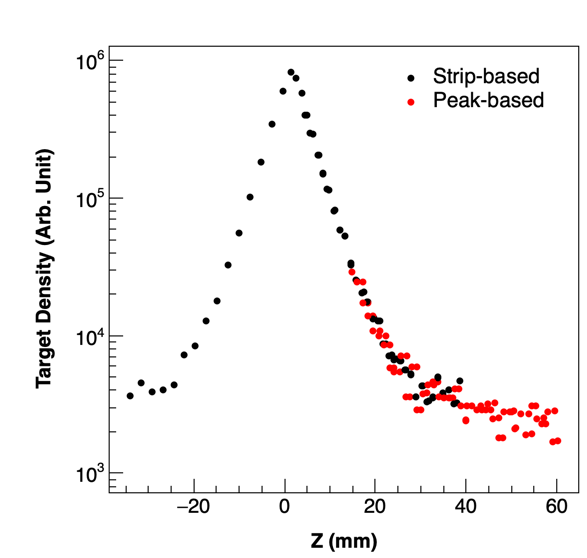
\includegraphics[width=0.35\textwidth]{./target_density_result.png}
  \caption{Target density profile measured at \SI{2.2}{\momentum}. The black
    data points are from the first method, the red data points are from the
    second method. They are aligned with each other with an offset of \SI{1.8}{\mm}.}
  \label{fig:target_density_result}
\end{figure}

\par
\medskip

%%%%% Discussion of the results
Fig. \ref{fig:target_density_result} shows the target density profile measured at
\SI{2.2}{\momentum}.
The distribution is almost symmetric with respect to the target center.
The main target body lies above a wide spread of residual gas distribution.
The main body of the target can be described by a double-gaussian model, with
\SI{43}{\percent} and \SI{57}{\percent} contribution from the narrow and wide
component respectively.
The narrow component has a $\sigma$ of \SI{2}{mm} and the wide one has a $\sigma$ of \SI{5.6}{mm}.
The overall FWHM of the target distribution is about \SI{6.9}{mm}.
The residual gas has a relatively uniform distribution over a wide region, even
beyond the recoil sensor's coverage.
The density of the residual gas is about 260 lower than the peak value of the
main target body, which proves the sensibility of this method (in comparison, the traditional
method using a rod probe of \SI{1}{\mm} diameter only has a sensibility of about
\SI{30}).

\par
\medskip

The measured target density distribution is much wider than the required design value
of \SI{2}{\mm} FWHM.
Correspondingly, the applibiltiy of the TOF-E selection method reaches its lower
limit at larger recoil angle than the design goal as well.
At \SI{2.2}{\momentum} beam momentum, the target body is not fully covered by
the forward detector starting from the strip Si1\_26.
This corresponds to the recoil energy of \SI{500}{\keV} and $|t| = \SI{0.001}{\tmom}$.
The background substraction method using the background model from strips which
are fully covered by the forward detector can extend the lower limit to $|t| = \SI{0.0008}{\tmom}$.
However, this method has larger systematic error than the TOF-E selection method.
Finally, to reach even lower $|t|$ range, new method needs to be developped to unfold the
actual event number from the partially-recorded energy spectrum.

\par
\medskip

%----------------------------------------------------------------
\begin{thebibliography}{99}
\bibitem{r1} Y. Zhou, Extraction of elastic scattering events in KOALA, IKP Annual Report 2021
\end{thebibliography}
\end{document}

